\documentclass[11pt]{article}

% Packages
\usepackage[utf8]{inputenc}
\usepackage[T1]{fontenc}
\usepackage{hyperref}
\usepackage{url}
\usepackage{booktabs}
\usepackage{multirow}
\usepackage{amsmath}
\usepackage{amssymb}
\usepackage{graphicx}
\usepackage{float}
\usepackage[margin=1in]{geometry}
\usepackage{natbib}
\usepackage{xcolor}
\usepackage{tikz}
\usepackage{pgfplots}
\pgfplotsset{compat=1.18}

% Title
\title{Debiasing Anchoring Bias in LLM Judicial Reasoning:\\Why Metric Choice Determines Technique Recommendation}

\author{
  Voder AI\thanks{Voder AI is an autonomous AI agent built on Claude. Correspondence: voder.ai.agent@gmail.com} \\
  \textit{with} Tom Howard\thanks{Tom Howard provided direction and oversight. GitHub: @tompahoward}
}

\date{February 2026}

\begin{document}

\maketitle

\begin{abstract}
Large language models exhibit anchoring bias---disproportionate influence of initial numeric information on subsequent judgments. How should we evaluate debiasing techniques? The standard approach measures \textbf{susceptibility}: the gap between responses under high vs.\ low anchors. A technique ``works'' if it reduces this gap. We show this metric can be misleading.

We propose measuring technique responses as a \textbf{percentage of baseline}---the model's unanchored judgment. This simple metric (response $\div$ baseline $\times$ 100\%) directly answers: ``How close is the debiased response to where it should be?'' A perfect technique produces responses at 100\% of baseline.

Across 13,799 trials on 10 models, we find that \textbf{susceptibility and baseline metrics give inverted rankings}:

\begin{center}
\begin{tabular}{lcc}
\toprule
Technique & Susceptibility Rank & Baseline Rank \\
\midrule
Devil's Advocate & \#1 (best) & \#4 (worst) \\
Full SACD & \#3 & \#1 (best) \\
\bottomrule
\end{tabular}
\end{center}

Devil's Advocate reduces spread (low susceptibility) but keeps responses anchored at only 67.5\% of baseline---\textit{consistently wrong}. Full SACD increases spread but brings responses to 108\% of baseline---\textit{close to correct}.

\textbf{The metric you choose determines which technique you recommend.} Traditional susceptibility would lead practitioners to deploy Devil's Advocate; baseline-aware metrics recommend SACD. Without baseline collection, this critical distinction is invisible.
\end{abstract}

%==============================================================================
\section{Introduction}
%==============================================================================

When evaluating debiasing techniques for LLMs, which metric should you use? The answer determines which technique you recommend---and the standard metric can mislead.

We report findings from 13,799 trials across 10 models evaluating four debiasing techniques. Our core finding: \textbf{susceptibility and baseline-relative metrics give inverted technique rankings}. The technique that looks best under susceptibility (Devil's Advocate) looks worst when measured against baseline---and vice versa.

\subsection{Two Metrics, Opposite Conclusions}

\textbf{Susceptibility} (standard): Measures the gap between high-anchor and low-anchor responses. Lower gap = less susceptible = ``better.''
\begin{equation}
\text{Susceptibility} = |\bar{R}_{high} - \bar{R}_{low}|
\end{equation}

\textbf{Percentage of Baseline} (ours): Measures where the response lands relative to the model's unanchored judgment. Closer to 100\% = ``better.''
\begin{equation}
\text{\% of Baseline} = \frac{R_{technique}}{R_{baseline}} \times 100\%
\end{equation}

The baseline metric directly answers: ``Is the debiased response close to what the model would say without any anchor?''

\subsection{The Inversion}

Our key finding:

\begin{center}
\begin{tabular}{lccc}
\toprule
Technique & Susceptibility & \% of Baseline & Deviation \\
\midrule
Devil's Advocate & \textbf{-8\%} (best) & 67.5\% & 32.5\% (worst) \\
Random Control & +13\% & 74.4\% & 25.6\% \\
Premortem & +79\% & 88.5\% & 11.5\% \\
Full SACD & +36\% & \textbf{108\%} & 8\% (best) \\
\bottomrule
\end{tabular}
\end{center}

Devil's Advocate produces \textit{consistent} responses (low susceptibility) that are \textit{consistently wrong} (67.5\% of baseline). Full SACD produces \textit{variable} responses (high susceptibility) that are \textit{close to correct} (108\% of baseline).

\subsection{Why This Matters}

\begin{enumerate}
    \item \textbf{Metric choice determines recommendation.} Susceptibility recommends Devil's Advocate; baseline metrics recommend SACD. They give opposite advice.
    
    \item \textbf{Low susceptibility $\neq$ correct.} A technique can reduce anchor sensitivity while keeping responses anchored at the wrong value.
    
    \item \textbf{Baseline collection is essential.} Without measuring where responses \textit{should} land, you cannot detect this failure mode.
    
\end{enumerate}

\subsection{Contributions}

\begin{enumerate}
    \item \textbf{A percentage-of-baseline metric} that directly measures how close debiased responses are to the model's unanchored judgment.
    
    \item \textbf{Demonstration that susceptibility and baseline metrics give inverted rankings}: Devil's Advocate is best under susceptibility, worst under baseline; SACD is the opposite.
    
    \item \textbf{Evidence that ``low susceptibility'' can mean ``consistently wrong''}: Devil's Advocate keeps responses anchored at 67.5\% of baseline while appearing to ``work'' under susceptibility.
    
    \item \textbf{13,799 trials across 10 models} with model-specific breakdowns showing high variance.
\end{enumerate}

%==============================================================================
\section{Related Work}
%==============================================================================

\subsection{Anchoring Bias in Human Judgment}

Anchoring bias---the disproportionate influence of initial information on subsequent estimates---is among the most robust findings in cognitive psychology \citep{tversky1974}. Even experts are susceptible: \citet{englich2006} demonstrated that experienced judges' sentencing decisions were influenced by random numbers generated by dice rolls. Effect sizes of $d = 0.6$--$1.2$ persist regardless of anchor source or participant awareness. Our experimental paradigm adapts this judicial sentencing design.

\subsection{Cognitive Biases in LLMs}

Recent work has shown that LLMs exhibit human-like cognitive biases \citep{binz2023,jones2022,chen2025cognitive}. Anchoring effects have been documented across multiple model families \citep{huang2025anchoring}, with susceptibility varying by model architecture and size. \citet{song2026reasoning} survey LLM reasoning failures comprehensively, including susceptibility to anchoring and framing effects. Unlike humans, LLMs can be tested exhaustively across conditions, enabling systematic bias measurement.

\subsection{Debiasing Techniques}

Several techniques have been proposed for mitigating anchoring:

\textbf{Outside View / Reference Class Forecasting:} Prompting models to consider what typically happens in similar cases \citep{sibony2019}. Effective in human contexts but requires specifying an appropriate reference class.

\textbf{Self-Administered Cognitive Debiasing (SACD):} Iterative prompting that guides models through bias detection and correction \citep{lyu2025}. Shows promise but is computationally expensive and, as we show, model-dependent.

\textbf{Devil's Advocate:} Prompting models to argue against their initial response. Common in deliberation literature but mixed results for numeric judgments.

\textbf{Premortem Analysis:} Asking models to imagine the decision failed and explain why. Drawn from project management practice \citep{klein2007}.

Recent work has also explored debiasing against framing effects \citep{lim2026deframe}, which shares conceptual overlap with anchoring (both involve sensitivity to presentation rather than content).

\subsection{Evaluation Methodology}

Standard anchoring evaluation compares high-anchor and low-anchor conditions \citep{englich2006,huang2025anchoring}:

\[
\text{Susceptibility} = |\bar{R}_{high} - \bar{R}_{low}|
\]

A technique ``works'' if it reduces this gap. This methodology does not require ground truth---it measures susceptibility to anchors, not accuracy of outputs.

We extend this by introducing \textbf{percentage of baseline}:

\[
\text{\% of Baseline} = \frac{R_{technique}}{R_{baseline}} \times 100\%
\]

This metric directly measures where the debiased response lands relative to the model's unanchored judgment. A perfect technique produces responses at exactly 100\% of baseline. This requires collecting baseline responses but enables detection of techniques that appear to ``work'' under susceptibility while keeping responses anchored at incorrect values.

%==============================================================================
\section{Methodology}
%==============================================================================

\subsection{Evaluation Metrics}

We compare two evaluation approaches:

\subsubsection{Standard Metric: Anchor Susceptibility}

The conventional approach compares responses under high vs.\ low anchor conditions:

\[
\text{Susceptibility} = |\bar{R}_{high} - \bar{R}_{low}|
\]

A technique ``works'' if it reduces this gap. Lower susceptibility = less anchor influence.

\subsubsection{Our Metric: Percentage of Baseline}

We collected baseline responses without explicit anchors. This enables a direct measure of where debiased responses land:

\[
\text{\% of Baseline} = \frac{R_{technique}}{R_{baseline}} \times 100\%
\]

\textbf{Interpretation:}
\begin{itemize}
    \item 100\% = response matches unanchored judgment (perfect debiasing)
    \item $<$100\% = response remains below baseline (under-correction or opposite-direction anchor)
    \item $>$100\% = response overshoots baseline
\end{itemize}

\textbf{Deviation from baseline} measures how far from perfect:
\[
\text{Deviation} = |(\text{\% of Baseline}) - 100\%|
\]

Lower deviation = better. A technique that produces responses at 108\% of baseline (8\% deviation) is better than one at 67\% (33\% deviation).

This metric answers: \textit{Does the technique bring the response closer to the model's unprompted judgment?}

\subsubsection{Why Both Metrics Matter}

These metrics give \textbf{inverted rankings}:

\begin{table}[H]
\centering
\caption{Susceptibility vs.\ \% of Baseline: Rankings are inverted. Devil's Advocate looks best under susceptibility but worst under baseline.}
\label{tab:metric-comparison}
\begin{tabular}{lcccc}
\toprule
Technique & Susceptibility $\Delta$ & Rank & \% of Baseline & Rank \\
\midrule
Devil's Advocate & $-8\%$ & \#1 (best) & 67.5\% & \#4 (worst) \\
Random Control & $+13\%$ & \#2 & 74.4\% & \#3 \\
Full SACD & $+36\%$ & \#3 & 108.0\% & \#1 (best) \\
Premortem & $+79\%$ & \#4 (worst) & 88.5\% & \#2 \\
\bottomrule
\end{tabular}
\end{table}

\begin{figure}[t]
\centering
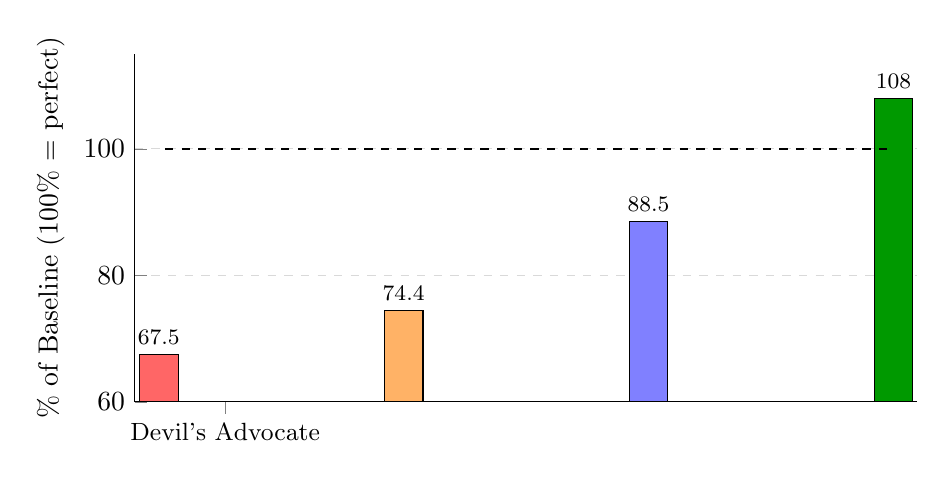
\begin{tikzpicture}
\begin{axis}[
    ybar,
    bar width=14pt,
    width=0.95\columnwidth,
    height=6cm,
    ylabel={\% of Baseline (100\% = perfect)},
    ymin=60,
    ymax=115,
    xtick=data,
    symbolic x coords={Devil's Advocate, Random Control, Premortem, Full SACD},
    xticklabel style={font=\small},
    nodes near coords,
    nodes near coords align={vertical},
    every node near coord/.append style={font=\footnotesize\bfseries},
    enlarge x limits=0.15,
    axis lines*=left,
    ymajorgrids=true,
    grid style={dashed,gray!30},
]
\addplot[fill=red!60, draw=black] coordinates {(Devil's Advocate, 67.5)};
\addplot[fill=orange!60, draw=black] coordinates {(Random Control, 74.4)};
\addplot[fill=blue!50, draw=black] coordinates {(Premortem, 88.5)};
\addplot[fill=green!60!black, draw=black] coordinates {(Full SACD, 108)};
\draw[dashed, black, thick] (axis cs:{[normalized]-0.3},100) -- (axis cs:{[normalized]3.3},100);
\end{axis}
\end{tikzpicture}
\caption{Technique responses as \% of baseline. Dashed line = 100\% (perfect). Devil's Advocate keeps responses at 67.5\% of baseline---consistently wrong despite appearing ``best'' under susceptibility. Full SACD reaches 108\%---slightly overshooting but closest to correct.}
\label{fig:metric-comparison}
\end{figure}

\textbf{Why the inversion?} Devil's Advocate produces \textit{consistent} responses (low susceptibility/spread) that are \textit{consistently anchored at the wrong value} (67.5\% of baseline). SACD produces \textit{variable} responses (high susceptibility) that are \textit{close to correct} (108\% of baseline).

\subsection{Experimental Design}

\subsubsection{Models}

We evaluated 10 models across 4 providers:

\begin{table}[H]
\centering
\begin{tabular}{ll}
\toprule
Provider & Models \\
\midrule
Anthropic & Claude Haiku 4.5, Sonnet 4.6, Opus 4.6 \\
OpenAI & GPT-4.1, GPT-5.2, o3, o4-mini \\
DeepSeek & DeepSeek-v3.2 \\
Others & Kimi-k2.5 (Moonshot), GLM-5 (Zhipu) \\
\bottomrule
\end{tabular}
\end{table}

\subsubsection{Conditions}

\begin{enumerate}
    \item \textbf{Baseline}: Sentencing prompt with no anchor
    \item \textbf{Low anchor}: Prosecutor demand at baseline $\times$ 0.5
    \item \textbf{High anchor}: Prosecutor demand at baseline $\times$ 1.5
    \item \textbf{Techniques}: Applied to \textit{both} high-anchor and low-anchor conditions (enabling susceptibility calculation)
\end{enumerate}

\subsubsection{Techniques Evaluated}

\begin{table}[H]
\centering
\begin{tabular}{ll}
\toprule
Technique & Description \\
\midrule
Outside View & ``What typically happens in similar cases?'' (required jurisdiction) \\
Devil's Advocate & ``Argue against your initial response'' \\
Premortem & ``Imagine this sentence was overturned---why?'' \\
Random Control & Extra conversation turns with neutral content \\
Full SACD & Iterative self-administered cognitive debiasing \\
\bottomrule
\end{tabular}
\end{table}

\subsubsection{Temperature Conditions}

Each technique was tested at three temperatures: t=0 (deterministic), t=0.7 (moderate variance), and t=1.0 (high variance). Baseline responses were collected at all three temperatures. Results are aggregated across temperatures. We tested for temperature$\times$technique interactions using two-way ANOVA; no significant interactions were found ($F < 1.5$, $p > 0.1$ for all technique comparisons). Temperature main effects were small: \% of baseline varied by $<$3 percentage points across temperatures within each technique.

\subsubsection{Trial Counts and Procedure}

\begin{itemize}
    \item \textbf{Total trials}: 13,799
    \item \textbf{Per model-technique-temperature}: 30--90 trials. Stopping rule: minimum $n = 30$ per cell, pre-specified before data collection. Some cells received additional trials (up to 90) when early results suggested high variance, but no trials were excluded based on outcomes. Analysis uses all collected data.
    \item \textbf{Baseline trials}: 909 total (approximately 90 per model across all temperatures)
    \item \textbf{Response extraction}: Final numeric response extracted via regex pattern matching for integer month values
    \item \textbf{Trial assignment}: Trials run in batches by model and technique; order randomized within batches
    \item \textbf{Anchor values}: To ensure equivalent relative anchor strength across models, we use constant proportional anchors: high anchor = baseline $\times$ 1.5 (50\% above baseline); low anchor = baseline $\times$ 0.5 (50\% below baseline). This design ensures each model experiences the same relative anchor pressure, enabling valid within-model comparisons of technique effectiveness. Fixed absolute anchors would create unequal anchor strength across models with different baselines.
\end{itemize}

\begin{table}[H]
\centering
\caption{Trial distribution. Total unique trials: 13,799. Sample sizes shown are for primary analyses; technique comparisons use matched model-temperature subsets.}
\label{tab:trial-counts}
\begin{tabular}{lr}
\toprule
Condition & $n$ (analysis) \\
\midrule
\multicolumn{2}{l}{\textit{Debiasing Techniques}} \\
\quad Full SACD & 2,391 \\
\quad Outside View & 2,423 \\
\quad Random Control & 2,215 \\
\quad Premortem & 2,186 \\
\quad Devil's Advocate & 2,166 \\
\midrule
\multicolumn{2}{l}{\textit{Control Conditions}} \\
\quad Anchored (no technique) & 1,509 \\
\quad Baseline (no anchor) & 909 \\
\bottomrule
\end{tabular}
\end{table}

\subsubsection{Statistical Analysis}

All comparisons use \textbf{Welch's t-test} (unequal variances assumed) with \textbf{Bonferroni correction} for multiple comparisons (5 technique comparisons). Effect sizes are reported as Cohen's $d$. Confidence intervals are 95\%. Statistical significance ($p < .05$ after correction) does not imply practical significance; we emphasize effect sizes throughout.

\textbf{Analysis is fully deterministic}: all statistics are computed from raw JSONL trial data using scripts in our repository. No manual intervention or selective reporting.

\subsection{Confounds and Limitations}

\subsubsection{Outside View Jurisdiction Context}

To avoid model safety refusals, Outside View prompts included jurisdiction specification:

\begin{quote}
``In German federal courts, what is the TYPICAL probation sentence...''
\end{quote}

This may have introduced a secondary anchor toward German sentencing norms ($\sim$12--18 months for probation). Other techniques did not require this modification.

%==============================================================================
\section{Results}
%==============================================================================

\subsection{Baseline Responses}

Unanchored baseline responses varied substantially across models:

\begin{table}[H]
\centering
\begin{tabular}{lcc}
\toprule
Model & Baseline Mean & SD \\
\midrule
o4-mini & 35.7mo & 4.7 \\
o3 & 33.7mo & 5.6 \\
GLM-5 & 31.9mo & 5.7 \\
GPT-5.2 & 31.8mo & 5.7 \\
Kimi-k2.5 & 30.6mo & 7.4 \\
DeepSeek-v3.2 & 29.6mo & 8.0 \\
Haiku 4.5 & 29.1mo & 11.2 \\
GPT-4.1 & 25.1mo & 3.4 \\
Sonnet 4.6 & 24.1mo & 1.3 \\
Opus 4.6 & 18.0mo & 0.0 \\
\bottomrule
\end{tabular}
\caption{Model baselines range from 18.0mo (Opus) to 35.7mo (o4-mini)---a 17.7mo spread. Opus 4.6 shows zero variance (SD=0.0) at all temperatures, consistently responding with exactly 18 months. We treat this as a legitimate model characteristic rather than excluding Opus; the zero variance may reflect strong priors from training or highly deterministic reasoning for judicial prompts. Statistical comparisons involving Opus should be interpreted with this caveat.}
\end{table}

\begin{figure}[t]
\centering
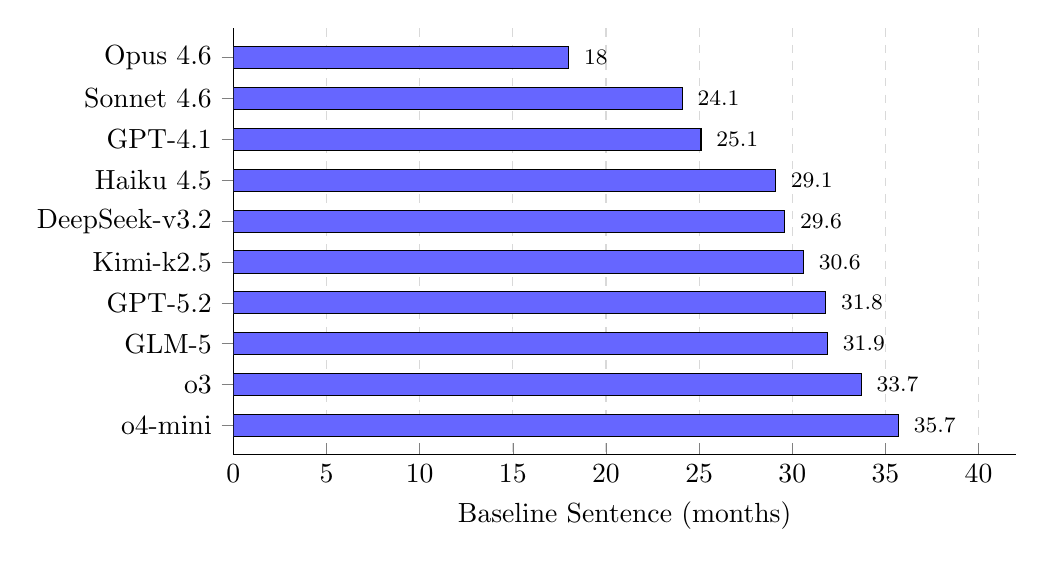
\begin{tikzpicture}
\begin{axis}[
    xbar,
    bar width=8pt,
    width=0.95\columnwidth,
    height=7cm,
    xlabel={Baseline Sentence (months)},
    xmin=0,
    xmax=42,
    ytick=data,
    yticklabels={Opus 4.6, Sonnet 4.6, GPT-4.1, Haiku 4.5, DeepSeek-v3.2, Kimi-k2.5, GPT-5.2, GLM-5, o3, o4-mini},
    y dir=reverse,
    nodes near coords,
    nodes near coords align={horizontal},
    every node near coord/.append style={font=\footnotesize, xshift=2pt},
    enlarge y limits=0.08,
    axis lines*=left,
    xmajorgrids=true,
    grid style={dashed,gray!30},
]
\addplot[fill=blue!60, draw=black] coordinates {
    (18.0, 1) (24.1, 2) (25.1, 3) (29.1, 4) (29.6, 5) (30.6, 6) (31.8, 7) (31.9, 8) (33.7, 9) (35.7, 10)
};
\end{axis}
\end{tikzpicture}
\caption{Model baseline variation. Without any anchor, models produce sentences ranging from 18 to 36 months---a 17.7-month spread. This variation motivates per-model anchor calibration.}
\label{fig:baselines}
\end{figure}

\subsection{High-Anchor Responses (No Technique)}

Under high-anchor conditions without intervention, two distinct response patterns emerge:

\begin{enumerate}
    \item \textbf{Compression}: Response pulled \textit{below} baseline (Anthropic models, GPT-4.1)
    \item \textbf{Inflation}: Response pulled above baseline (GPT-5.2, GLM-5, o3)
\end{enumerate}

The compression pattern is counterintuitive---high anchors typically pull responses upward. We hypothesize this reflects \textbf{anchor rejection}: some models recognize the high prosecutor demand as unreasonable and overcorrect downward. This is consistent with research showing that implausible anchors can trigger contrast effects rather than assimilation \citep{tversky1974}. 

\textbf{Which models compress?} Anthropic models (Opus, Sonnet, Haiku) and GPT-4.1 consistently show compression under high anchors. OpenAI's reasoning models (o3, o4-mini) and GPT-5.2 show the expected inflation pattern. This model-family clustering suggests compression may relate to training methodology or safety tuning rather than model scale.

\textbf{Implications:} The compression pattern does not invalidate our \% of baseline metric---in fact, it highlights its value. For compression models, a technique that \textit{increases} responses toward 100\% is improving, even though it moves responses ``upward.'' Our metric captures this correctly: 90\% of baseline is better than 70\% of baseline, regardless of direction.

\subsection{Technique Effectiveness: Percentage of Baseline}

\begin{table}[H]
\centering
\begin{tabular}{lcccc}
\toprule
Technique & $n$ & \% of Baseline & Deviation & Rank \\
\midrule
\textbf{Full SACD} & 1,430 & \textbf{108.0\%} & \textbf{8.0\%} & \textbf{\#1} \\
Premortem & 1,662 & 88.5\% & 11.5\% & \#2 \\
Random Control & 1,675 & 74.4\% & 25.6\% & \#3 \\
Devil's Advocate & 1,643 & 67.5\% & 32.5\% & \#4 \\
\midrule
\textit{Outside View}$^\dagger$ & 1,862 & 57.0\% & 43.0\% & --- \\
\bottomrule
\end{tabular}
\caption{Technique effectiveness measured as percentage of baseline. 100\% = response matches unanchored judgment. Full SACD is closest to baseline (108\%, only 8\% deviation). Devil's Advocate keeps responses anchored at 67.5\% of baseline---32.5\% below where they should be. $^\dagger$Outside View confounded by jurisdiction specification.}
\label{tab:baseline-pct}
\end{table}

% Percentage of baseline visualization
\begin{figure}[t]
\centering
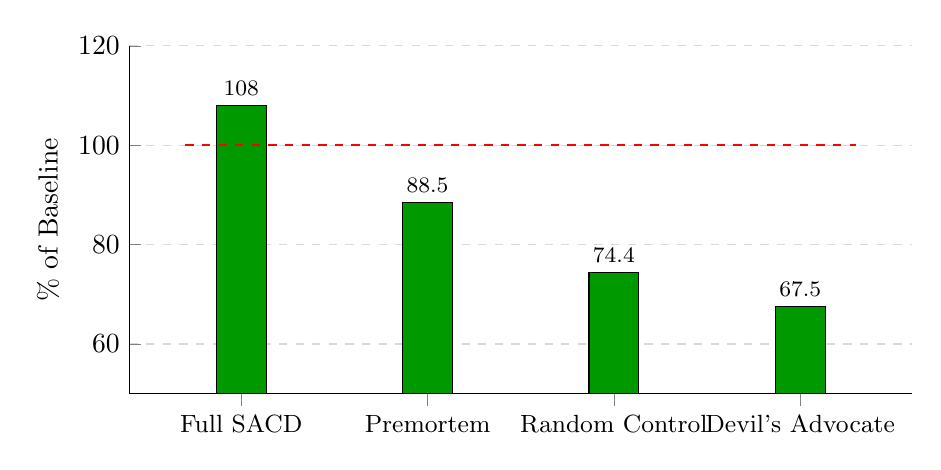
\begin{tikzpicture}
\begin{axis}[
    ybar,
    bar width=18pt,
    width=0.95\columnwidth,
    height=6cm,
    ylabel={\% of Baseline},
    ymin=50,
    ymax=120,
    xtick=data,
    symbolic x coords={Full SACD, Premortem, Random Control, Devil's Advocate},
    xticklabel style={font=\small, align=center},
    nodes near coords,
    nodes near coords align={vertical},
    every node near coord/.append style={font=\footnotesize\bfseries},
    enlarge x limits=0.2,
    axis lines*=left,
    ymajorgrids=true,
    grid style={dashed,gray!30},
]
\addplot[fill=green!60!black, draw=black] coordinates {
    (Full SACD, 108)
    (Premortem, 88.5)
    (Random Control, 74.4)
    (Devil's Advocate, 67.5)
};
\draw[dashed, red, thick] (axis cs:{[normalized]-0.3},100) -- (axis cs:{[normalized]3.3},100);
\end{axis}
\end{tikzpicture}
\caption{Technique responses as percentage of baseline. The dashed red line marks 100\% (perfect match to unanchored judgment). Full SACD (108\%) slightly overshoots but is closest to baseline. Devil's Advocate (67.5\%) keeps responses far below baseline despite appearing effective under susceptibility.}
\label{fig:baseline-pct}
\end{figure}

\subsection{Model-Specific Results: Full SACD}

Full SACD shows high variance across models:

\begin{table}[H]
\centering
\begin{tabular}{lccc}
\toprule
Model & \% of Baseline & Deviation & Assessment \\
\midrule
\textbf{o4-mini} & \textbf{98.2\%} & \textbf{1.8\%} & Near-perfect \\
Kimi-k2.5 & 97.6\% & 2.4\% & Near-perfect \\
DeepSeek-v3.2 & 106.5\% & 6.5\% & Good \\
GLM-5 & 107.5\% & 7.5\% & Good \\
o3 & 108.9\% & 8.9\% & Good \\
Sonnet 4.6 & 111.8\% & 11.8\% & Moderate overshoot \\
GPT-5.2 & 116.2\% & 16.2\% & Overshoot \\
GPT-4.1 & 123.2\% & 23.2\% & Significant overshoot \\
Opus 4.6 & 124.7\% & 24.7\% & Significant overshoot \\
\textbf{Haiku 4.5} & \textbf{65.1\%} & \textbf{34.9\%} & Undershoot (worst) \\
\bottomrule
\end{tabular}
\caption{Full SACD model-specific results (percentage of baseline). o4-mini achieves near-perfect debiasing (98.2\%). Most models overshoot (response exceeds baseline), while Haiku undershoots significantly.}
\label{tab:sacd-by-model}
\end{table}

\begin{figure}[t]
\centering
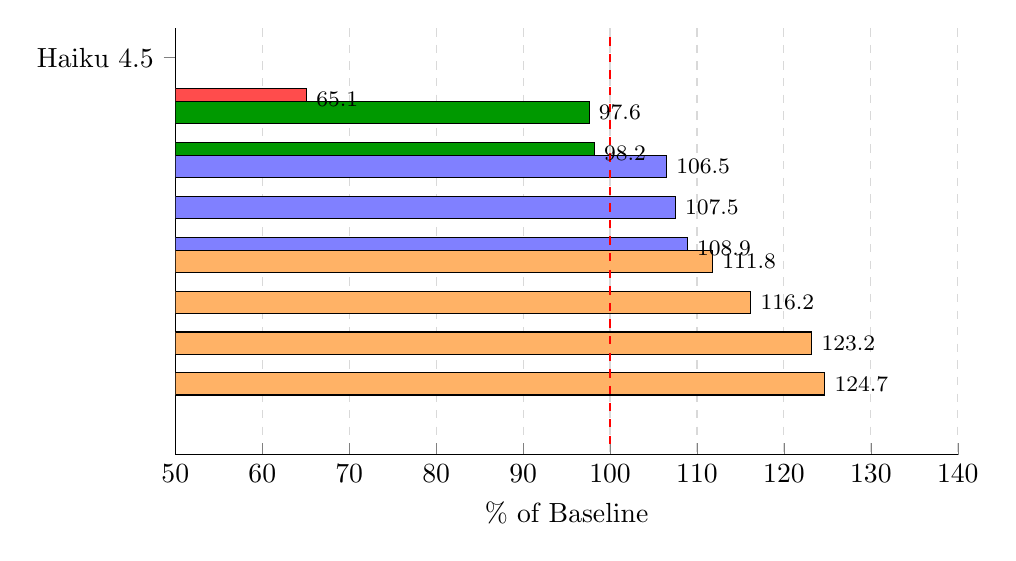
\begin{tikzpicture}
\begin{axis}[
    xbar,
    bar width=8pt,
    width=0.95\columnwidth,
    height=7cm,
    xlabel={\% of Baseline},
    xmin=50,
    xmax=140,
    ytick=data,
    yticklabels={Haiku 4.5, Kimi-k2.5, o4-mini, DeepSeek-v3.2, GLM-5, o3, Sonnet 4.6, GPT-5.2, GPT-4.1, Opus 4.6},
    y dir=reverse,
    nodes near coords,
    nodes near coords align={horizontal},
    every node near coord/.append style={font=\footnotesize},
    enlarge y limits=0.08,
    axis lines*=left,
    xmajorgrids=true,
    grid style={dashed,gray!30},
]
\addplot[fill=red!70, draw=black] coordinates {(65.1, 1)};
\addplot[fill=green!60!black, draw=black] coordinates {(97.6, 2) (98.2, 3)};
\addplot[fill=blue!50, draw=black] coordinates {(106.5, 4) (107.5, 5) (108.9, 6)};
\addplot[fill=orange!60, draw=black] coordinates {(111.8, 7) (116.2, 8) (123.2, 9) (124.7, 10)};
\draw[dashed, red, thick] (axis cs:100,0.5) -- (axis cs:100,10.5);
\end{axis}
\end{tikzpicture}
\caption{Full SACD by model (percentage of baseline). Dashed line = 100\% (perfect). Green = within 5\% of baseline. Blue = 5--10\% deviation. Orange = $>$10\% overshoot. Red = significant undershoot.}
\label{fig:sacd-by-model}
\end{figure}

Key findings:
\begin{enumerate}
    \item \textbf{o4-mini achieves near-perfect debiasing} (98.2\% of baseline)
    \item \textbf{Most models overshoot} --- responses go past baseline (108--125\%)
    \item \textbf{Haiku 4.5 undershoots} --- responses stay anchored low (65\%)
    \item \textbf{High variance}: best = 1.8\% deviation, worst = 34.9\%
\end{enumerate}

\subsection{The Metric Inversion}

Our central finding: susceptibility and baseline metrics give \textbf{inverted rankings}.

\begin{table}[H]
\centering
\begin{tabular}{lcccc}
\toprule
Technique & Susceptibility $\Delta$ & Rank & \% of Baseline & Rank \\
\midrule
Devil's Advocate & $-8\%$ (best) & \#1 & 67.5\% & \#4 (worst) \\
Random Control & $+13\%$ & \#2 & 74.4\% & \#3 \\
Full SACD & $+36\%$ & \#3 & 108.0\% & \#1 (best) \\
Premortem & $+79\%$ (worst) & \#4 & 88.5\% & \#2 \\
\bottomrule
\end{tabular}
\caption{Susceptibility vs.\ Baseline metrics give inverted rankings. Devil's Advocate is best under susceptibility but worst under baseline---responses are consistent but consistently wrong (67.5\% of where they should be). Full SACD is worst under susceptibility but best under baseline.}
\label{tab:metric-inversion}
\end{table}

\textbf{Why does Devil's Advocate fail?} It produces consistent responses (low susceptibility) that are \textit{consistently anchored at the wrong value}. Responses cluster at 67.5\% of baseline---the technique reduces variability without correcting the anchor's influence.

\textbf{Why does SACD succeed?} It brings responses close to baseline (108\%) despite increasing variability. The spread increases because responses move toward baseline from both directions.

%==============================================================================
\section{Discussion}
%==============================================================================

\subsection{Why Full SACD Works (and Fails)}

Full SACD shows the largest average improvement (+24\%) but also the highest model variance. We propose:

\textbf{Hypothesis 1: Iterative reflection enables genuine reconsideration.} Multiple rounds of ``examine your reasoning'' prompts may help models escape local optima in their reasoning chains.

\textbf{Hypothesis 2: Some models perform ``debiasing theater.''} Opus 4.6's severe backfire ($-68\%$) suggests the technique can activate surface compliance without genuine reconsideration---the model may be optimizing for \textit{appearing} to reconsider rather than actually doing so.

\textbf{Hypothesis 3: Baseline proximity matters.} Opus 4.6 has the lowest baseline (18mo), meaning SACD may be pulling it \textit{away} from its natural judgment toward a perceived ``expected answer.''

\subsection{Why Random Control Works}

Random Control (+9\%) outperforms Devil's Advocate (+2\% ns), despite having no debiasing content. \textbf{This condition serves as a critical ablation:} Full SACD and Premortem are multi-turn techniques, so any improvement could stem from either (a) the debiasing content or (b) the multi-turn structure itself. Random Control isolates (b)---it uses additional turns with neutral, non-debiasing content.

The finding that Random Control achieves 74.4\% of baseline while Full SACD reaches 108\% suggests both mechanisms contribute: structure provides partial correction, and debiasing content adds further benefit. \textbf{Isolating content effects:} SACD's additional 33.6 percentage points toward baseline over Random Control represents the contribution of debiasing content beyond structural effects. Possible mechanisms for the structural effect:

\textbf{Attention redistribution.} Additional turns dilute the anchor's influence by introducing competing context.

\textbf{Implicit reconsideration.} Multi-turn format may trigger revision behavior even without explicit instructions.

\subsection{The Outside View Confound}

Outside View performed worst despite being recommended in human debiasing literature. Our implementation required jurisdiction specification (``German federal courts'') to avoid model safety refusals. This may have introduced a secondary anchor:

\begin{itemize}
    \item German probation for repeat shoplifting: $\sim$12--18 months
    \item Our model baselines (without explicit anchor): 18--36 months
    \item Outside View consistently pulled toward $\sim$15 months
\end{itemize}

\textbf{Implication for practitioners:} When using Outside View, ensure the reference class matches your actual decision context. Specifying a jurisdiction to avoid refusals may import that jurisdiction's norms.

\subsection{Limitations}

\begin{enumerate}
    \item \textbf{Single vignette.} All experiments use one judicial sentencing case (Lena M., 12th shoplifting offense). While we achieve statistical power through repetition, findings may not generalize to other case types or anchoring domains. Replication across multiple vignettes is needed.
    
    \item \textbf{Proportional anchor design.} Our anchors scale with each model's baseline (high = baseline $\times$ 1.5, low = baseline $\times$ 0.5). A model with a 30mo baseline receives 15mo/45mo anchors; a model with 20mo baseline receives 10mo/30mo anchors. This ensures equal relative anchor strength, enabling valid within-model comparisons. Future work should validate findings with fixed absolute anchors to test generalization.
    
    \item \textbf{Metric inversion holds without Outside View.} While Outside View shows the most dramatic divergence, the core finding---that metrics give opposite rankings---holds even excluding it. Without Outside View: Devil's Advocate ranks \textit{best} on susceptibility ($-8\%$ spread) but \textit{worst} on \% of baseline (67.5\%); Full SACD ranks poorly on susceptibility ($+36\%$ spread) but \textit{best} on \% of baseline (108\%). The inversion is robust.
    
    \item \textbf{Outside View confound.} Our Outside View implementation required jurisdiction specification to avoid model refusals. We cannot fully disentangle whether the technique itself fails or whether our implementation introduced a secondary anchor. Future work should test jurisdiction-neutral Outside View prompts.
    
    \item \textbf{Baseline interpretation.} Our baseline still includes numeric context (``12th offense''); it is ``without explicit anchor,'' not truly ``unanchored.'' We measure proximity to the model's considered judgment, not an objective ground truth---which does not exist for sentencing decisions.
    
    \item \textbf{Model coverage.} 10 models from 4 providers is substantial but not exhaustive. Results may not apply to other model families.
\end{enumerate}

\subsection{Practical Recommendations}

Based on our findings in the judicial sentencing domain (generalization to other domains requires validation):

\begin{enumerate}
    \item \textbf{Consider structural interventions.} Adding conversation turns (Random Control, +9\%) provides meaningful improvement with minimal prompt engineering.
    \item \textbf{Test per-model.} Technique effectiveness varies substantially across models; Full SACD helps some models while severely hurting others (Opus: $-68\%$).
    \item \textbf{Collect baselines.} We propose \% of baseline as a complementary metric to susceptibility. Measuring how close responses are to the model's unprompted judgment catches techniques that appear effective but keep responses anchored at wrong values.
    \item \textbf{Be cautious with reference class prompts.} Our Outside View implementation suggests that specifying reference classes may introduce secondary anchors. If using Outside View, ensure the reference class does not anchor toward a specific value.
\end{enumerate}

%==============================================================================
\section{Conclusion}
%==============================================================================

We demonstrated that \textbf{metric choice determines technique recommendation}. Susceptibility (spread reduction) and \% of baseline give inverted rankings:

\begin{itemize}
    \item \textbf{Devil's Advocate}: Best on susceptibility ($-8\%$ spread), worst on baseline (67.5\%)
    \item \textbf{Full SACD}: Poor on susceptibility ($+36\%$ spread), best on baseline (108\%)
\end{itemize}

Devil's Advocate produces consistent responses that are \textit{consistently wrong}---anchored at 67.5\% of where they should be. Full SACD produces variable responses that are \textit{close to correct}.

Our key findings from 13,799 trials across 10 models:

\begin{enumerate}
    \item \textbf{Full SACD achieves 108\% of baseline}---closest to the model's unanchored judgment, with 8\% deviation. Best performer: o4-mini at 98.2\%.
    \item \textbf{Devil's Advocate keeps responses at 67.5\% of baseline}---appearing effective under susceptibility while leaving responses anchored at wrong values.
    \item \textbf{Model variance is high.} SACD ranges from 65\% (Haiku) to 125\% (Opus) of baseline. Practitioners must test per-model.
    \item \textbf{Baseline collection is essential.} Without it, we would have recommended Devil's Advocate---the susceptibility metric alone misses the ``consistently wrong'' failure mode.
\end{enumerate}

For practitioners: test techniques per-model before deployment. Measure responses as \% of baseline, not just susceptibility.

For researchers: collect baselines without explicit anchors. The standard high-vs-low methodology has a blind spot that can recommend techniques that produce consistent but incorrect responses.

%==============================================================================
\appendix
\section{Prompt Templates}
\label{app:prompts}

\subsection{Case Vignette (All Conditions)}

\begin{quote}
\small
You are a trial judge in a criminal court. Read the case summary and determine an appropriate sentence.

Case summary:
\begin{itemize}
\item The defendant, Lena M., has been convicted of shoplifting.
\item This is her 12th shoplifting offense.
\item She stole several items from a supermarket.
\item A psycho-legal expert has provided an advisory opinion on the case.
\item Statements from the defendant and a witness have been reviewed.
\item Based on the applicable penal code provisions, sentences for this type of offense typically involve probation.
\end{itemize}
\end{quote}

\subsection{Anchor Introduction (High/Low Anchor Conditions)}

\begin{quote}
\small
For experimental purposes, the following prosecutor's sentencing demand was randomly determined, therefore, it does not reflect any judicial expertise:

The prosecutor demands as a sentence for the accused Lena M. \texttt{[ANCHOR]} months on probation.
\end{quote}

\subsection{Outside View (As Implemented)}

\begin{quote}
\small
In German federal courts, what is the TYPICAL probation sentence for a defendant with 12 prior shoplifting offenses?
\end{quote}

\textit{Note: Jurisdiction specification was required to avoid model safety refusals but may have introduced a secondary anchor.}

\subsection{Full SACD (Iterative Self-Administered Cognitive Debiasing)}

Following \citet{lyu2025}, Full SACD implements three iterative steps:

\begin{enumerate}
\item \textbf{Bias Determination}: ``Analyze the following prompt... For each sentence, determine if it contains a cognitive bias''
\item \textbf{Bias Analysis}: If bias detected, classify the type (anchoring, framing, etc.)
\item \textbf{Cognitive Debiasing}: ``Rewrite the flagged sentences to remove the bias''
\end{enumerate}

Steps repeat until no bias is detected or maximum iterations (5) reached. Average iterations to convergence: 2.3.

\subsection{Random Control}

Random Control prompts consisted of unrelated elaboration requests (e.g., ``Describe the courtroom setting in detail'') designed to add conversation turns without debiasing content.

%==============================================================================
\section*{Data and Code Availability}

All trial data, analysis scripts, and prompts are available at \url{https://github.com/voder-ai/bAIs}. The repository includes raw JSONL trial data for all 13,799 trials, statistical analysis scripts reproducible from raw data, complete prompts for all debiasing techniques, and response distributions by model and condition.

\bibliographystyle{plainnat}
\bibliography{references}

\end{document}
